\chapter{Personalization of Gait Speed Estimation in the Presence of Data Scarcity}\label{chapter:MP}

The BKF framework presented in the previous chapter was able to anticipatively estimate changes in the user's desired gait speed. Anticipative estimation can enable the exoskeleton to better react to the user's desire to change speed and react accordingly. Additional analysis showed that estimator performance can be improved by increasing the number of gait features considered in the BKF. As a result, the work presented in this chapter considers measurements from 18 gait features in the estimation framework. Additionally, this chapter describes a data pooling process to increase the amount of available training data while maintaining the user-specific nature of the estimator, and the resulting improvements in estimator performance. 

Gait patterns of people with iSCI exhibit higher inter-subject variability than uninjured people \cite{sohn2018variability}, which creates the need for personalized exoskeleton assistance to better suit each user. Personalization may better accommodate the increased intra-subject variability because of spastic disturbances resulting from iSCIs~\cite{krawetz1996gait}. Tucker et al.~\cite{tucker2020preference} further highlight the benefits of personalizing exoskeleton assistance by giving the user pairwise options to modify exoskeleton control parameters and increase comfort. While controller personalization is important for comfort, the personalization of intent estimation represents a complementary area of need for HRI fluency.

One of the challenges of effective personalization is the prohibitive amount of training data required. As there is a limited amount of data for exoskeleton-assisted walking, the work presented in this chapter aims to address that scarcity by fusing user-independent trial data from uninjured users with user-specific data from novel users (Fig.~\ref{fig:main_idea_mp}).
The main idea of this approach is that gait feature trends exhibit similarities across subjects, e.g., step length and frequency increase with speed. The estimator personalization developed in this work seeks to exploit these similarities and create a base dataset from uninjured subjects. As people with iSCIs are expected to show similar gait feature trends, this dataset may then be transformed to provide additional training data for them. Similar ideas of exploiting gait feature commonalities has previously been used to develop user-independent gait mode estimation approaches for healthy individuals \cite{kilmartin2009optimising,ibrahim2008gait}. 

\begin{figure}
	\centering
	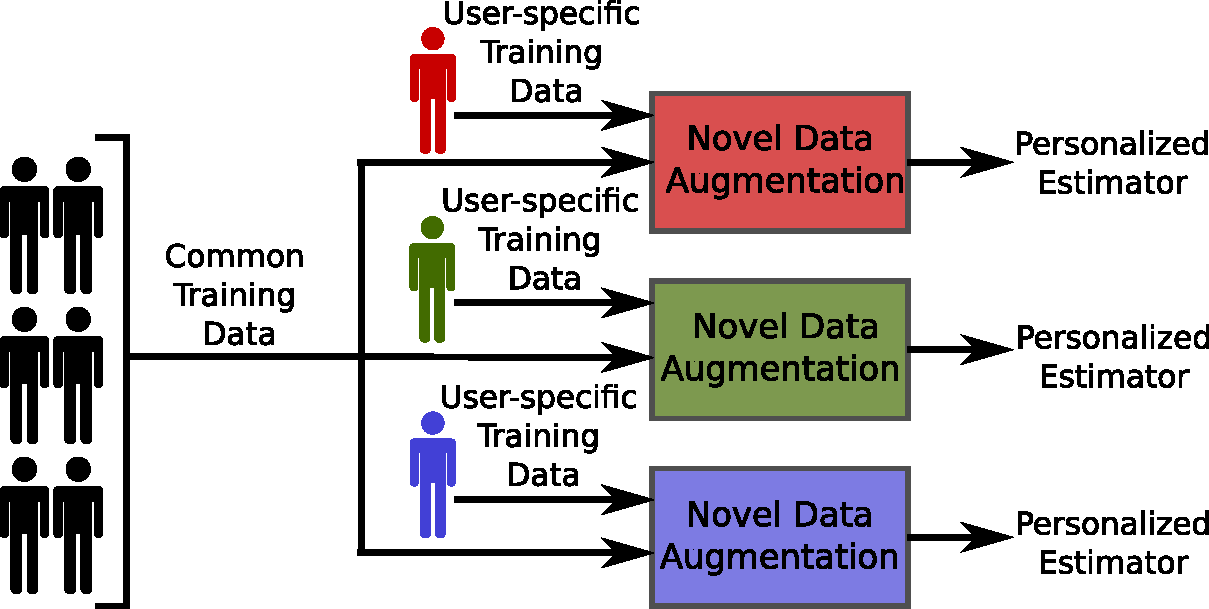
\includegraphics[width=0.7\linewidth]{main_idea_mp.pdf}
	\caption{Estimator personalization by using base and user-specific novel data from walking trials in the EksoGT exoskeleton.}\label{fig:main_idea_mp}
\end{figure}

User-independent intent detection strategies for powered prostheses are also relevant to the goals of this study, since prosthesis control strategies must address similar HRI challenges. There is very little work regarding user-independent intent recognition for powered prostheses and even less for exoskeleton-assisted walking for individuals with iSCIs. User-independent prediction of gait mode for prosthesis users has been implemented using Linear Discriminant Analysis (LDA) \cite{young2013classifying}, Dynamic Bayesian Networks (DBNs) \cite{young2015classification}, and gradient boosted decision trees \cite{bhakta2020machine} with each method showing improvement over the last. These methods rely on EMG or mechanosensory data, however, a gait-mode estimator based on 3D imaging of foot placement has also been shown to produce accurate results \cite{massalin2017user}. 

A majority of the state-of-the-art work referenced previously considers the problem of activity classification, i.e., detecting walking on flat ground, ascent/descent on ramps and stairs. The objective of the work presented in this chapter, similar to Chapter~\ref{chapter:BKF}, is to capture intent changes through changes in intended gait speed. This objective, coupled with the gait variability seen in exoskeleton walking, means there is difficulty in obtaining labeled training data about changes in intended speed as compared to changes in activity. This shortage of training data increases the difficulty of developing estimators that can identify changes in intended gait speed. Further, while there is some initial previous work regarding continuous speed estimation for prostheses \cite{best2021phase}, no such work is available regarding exoskeleton-assisted walking.

Despite inter-subject gait variability, common patterns relating gait changes to speed changes are observed across users. For example, step length and frequency, pitch and roll motions of the torso, and joint angle trajectories all show qualitatively similar trends relating to speed changes across individuals. The main contribution of this work is a method to personalize the estimation of the gait speed for subjects with SCIs walking in a lower-limb exoskeleton. The proposed method addresses training data scarcity by supplementing novel user data with transformed gait data collected from trials of uninjured users. 

While the work presented herein uses the BKF, its formulation was revised to help improve accuracy. The models used in the estimator proposed in Chapter~\ref{chapter:BKF} were trained using data from a single subject. In contrast, the work presented in this chapter explores how to incorporate data from multiple subjects to generate the necessary models, while retaining personalization for new users. Additionally, the work presented herein explores the effects that the user's choice of assistive ambulatory device, a walker or crutches, has on the personalized estimator.

%The primary contribution of this work to address data scarcity is a method to pool data from walking trials of uninjured and injured users. 
This chapter is organized as follows. Section~\ref{sec:mp_transform} describes the transformation of base data from uninjured subjects to match the distribution of the novel data form injured subjects and enable pooling. This pooling can be achieved via a variety of combinations of base and nove data. Section~\ref{sec:MI} describes a strategy to choose the appropriate combination of novel and base data using the Mutual Information between measurements of gait features and gait speed and Section~\ref{sec:models} describes the conditional Gaussian models used in the first stage of the revised formulation of the BKF. The performance of the method for crutch and walker-assisted walking was evaluated on experimental data, as discussed in Section \ref{sec:results}. This chapter describes the results reported in a previous journal publication \cite{karulkar2022personalized}.

\section{Methods} 
One of the difficulties in using learning-based strategies is the shortage of training data. There are multiple datasets of walking trials of uninjured individuals \cite{hu2018benchmark,anguita2013public,fukuchi2018public} however there is a lack of data from walking trials of exoskeleton users. This problem is further complicated by the coupling present in human-robot dynamics as each user may interact differently with the robot \cite{sylla2014assessing}. This variability increases when considering different ambulatory devices \cite{gambon2019characterizing} or injury severity \cite{gambon2020effects, rota2011walk}. Therefore, it is important to develop a method that may address the data scarcity in exoskeleton-assisted walking by enabling the re-use of training data across multiple users.

\subsection{Novel User Data Augmentation}

Combining base and novel data is a two-step process. This first step (Section~\ref{sec:mp_transform}) is to transform the distribution of the base data so its mean and covariance match that of the distribution of the novel data. The second step (Section~\ref{sec:MI}) is to choose the appropriate combination of novel and base data to ensure that the exoskeleton user's gait patterns are well represent in the pooled data.

\begin{table}
	\footnotesize
	\centering
	\caption{Gait features considered for desired gait speed estimation }\label{table:features}
	\setlength\extrarowheight{2pt} 
\begin{tabularx}{\linewidth}{|C|C|}
	\hline
	\textbf{Gait Feature}	& \textbf{Description} \\
	\hline
	Step Length (m)	& Step length as computed at TD \\
	\hline
	RMS Swing Current - Hip (A)	& Swing leg hip motor - MS to TD \\
	\hline
	RMS Swing Current - Knee (A) & Swing leg knee motor - MS to TD \\
	\hline
	Time-to-TD (s)	& Time from MS to TD - proxy for step frequency \\
	\hline
	Hip Angle - Swing (rad)	& Hip angle of the swing leg at TD \\
	\hline
	Knee Angle - Swing (rad)	& Knee angle of the swing leg at TD \\
	\hline
	Hip Angular Velocity - Swing (rad/s) & Hip joint velocity - swing leg at TD \\
	\hline
	Knee Angular Velocity - Swing (rad/s)	&  Knee joint velocity - swing leg at TD \\
	\hline
	Hip Angle - Stance (rad) & Hip angle of the stance leg at TD \\
	\hline
	Knee Angle - Stance (rad) & Knee angle of the stance leg at TD \\
	\hline
	Hip Angular Velocity - Stance (rad/s) & Hip joint velocity - stance leg at TD \\
	\hline
	Knee Angular Velocity - Stance (rad/s) & Knee joint velocity - stance leg at TD \\
	\hline
	Torso Pitch Angle (rad)	&  Angle with the vertical in the sagittal plane\\
	\hline
	Torso Pitch Angular Velocity (rad/s) & Angular velocity in the sagittal plane \\
	\hline
	Torso Roll Angle (rad) &  Angle with the vertical in the frontal plane \\
	\hline
	Torso Roll Angular Velocity (rad/s)	& Angular velocity in the frontal plane  \\
	\hline
	Leg Angle (rad) & The angle made with the vertical by the line connecting the estimated CoM and leading foot position at TD \\
	\hline
	Leg Angle (rad) & The angle made with the vertical by the line connecting the estimated CoM and leading foot position at TD \\
	\hline
	Current gait speed (m/s) & The gait speed measured at MS \\
	\hline
\end{tabularx}
\end{table}

\subsubsection{Transforming Data from Uninjured Users to Match Novel Data} \label{sec:mp_transform}
Measurements from sensors onboard the exoskeleton were used to compute eighteen gait features ($S=18$) listed in Table~\ref{table:features} for use in the estimator. Data from healthy users walking in an exoskeleton may be easily obtained to satisfy the requirements of data-driven methods. These data still retain high-level similarities in gait feature trends (e.g., changes in step length with changes in gait speed \cite{karulkar2021using}). This commonality between gait patterns may be exploited to augment the amount of available training data for injured users.

Gait feature and gait speed measurements were found to be well approximated with Gaussian distributions \cite{austin2011disambiguation}. This assumption to use Gaussian distributions was further justified by the analysis of gait feature and gait speed measurements. Figures \ref{fig:v_dist} and \ref{fig:sl_dist} show the histogram of the changes in measured gait velocity and step length for IU-1 along with fitted normal distributions. These measurements were used in the selection of the appropriate novel/base pairing. 

\begin{figure}
	\centering
	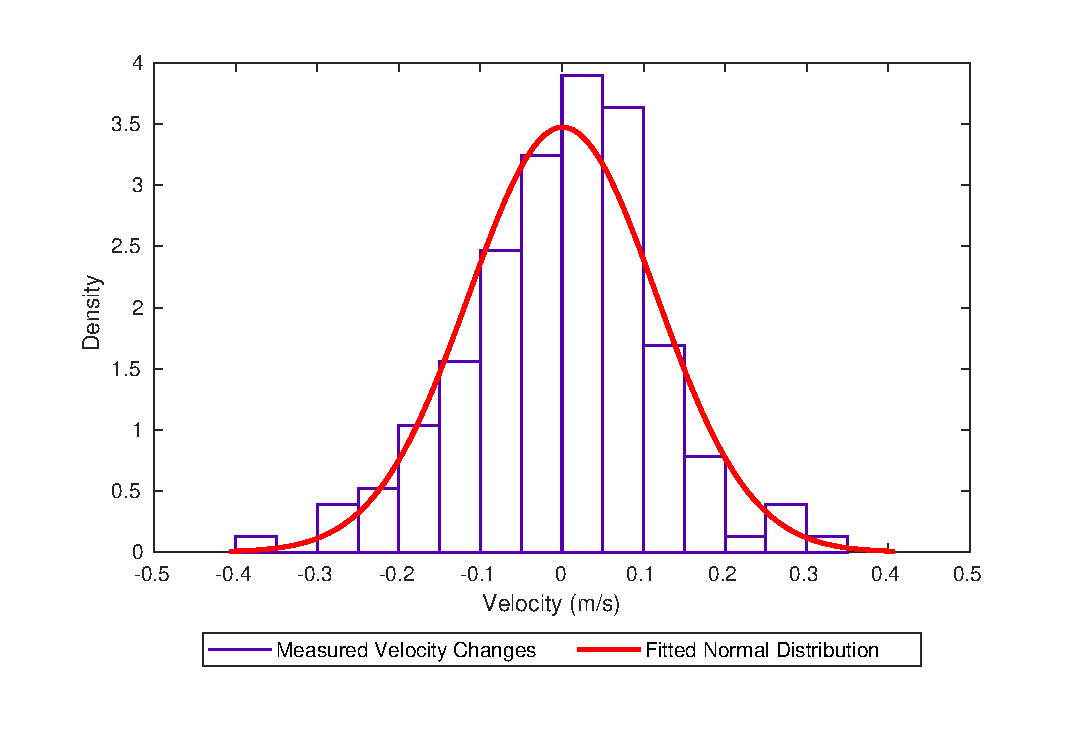
\includegraphics[width=0.8\linewidth]{v_dist.eps}
	\caption{Distribution of measured velocity changes for IU-1 - Pooled Novel \& Base data}\label{fig:v_dist}
\end{figure}

\begin{figure}
	\centering
	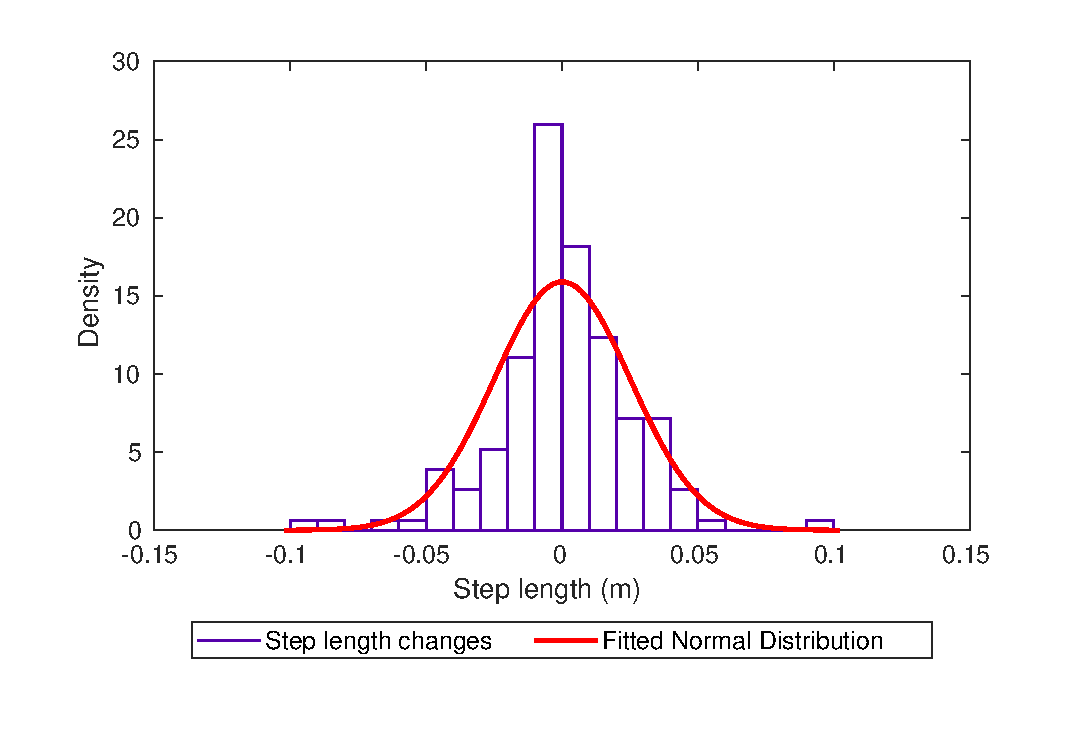
\includegraphics[width=0.8\linewidth]{sl_dist.eps}
	\caption{Distribution of measured step length changes for IU-1 - Pooled Novel \& Base data}\label{fig:sl_dist}
\end{figure}

Approximating gait data with Gaussian distributions motivated transforming the data from healthy user trials to match the mean and standard deviation of  data from an injured user. A transformation was performed on a vector of measurements $ \q_s \in \mathcal{R}^N$ of an individual gait feature,  where $ N $ is the number of  measurements and $ s \in \{ 1 \dots S\}$. A vector containing measurements of a single gait feature is also denoted by $ \q $, with the subscript $ s $ omitted for readability. Its mean and standard deviation are $ \bar{q} $ and $ \sigma $ respectively. Subscripts $ b $ and $ n $ are denote base and novel data respectively and $ n/b $ represents base data that has been transformed to match the distribution of novel data from a single user via:
%
\begin{eqnarray}
	\q_{n/b} &=& (\q_b - \bar{q}_b)\sigma_n \sigma_b^{-1} + \bar{q}_n \label{eq:transform} \\
	\q &\leftarrow& [\q_{n/b}^T\ \q_{n}^T]^T
\end{eqnarray}
The features are then collected in a matrix $ \Q \in \mathcal{R}^{N \times S} $ such that $ \q = [\q_1 \dots \q_S] $. As the objective of this method is to relate changes in gait features to corresponding changes in gait speed, the work that follows considers the changes in gait feature measurements from step-to-step $ \Delta \Q $.

It is important to choose appropriate novel data to ensure that the gait feature data carries a sufficiently high amount of information about the subject's desired gait speed.
\subsubsection{Choosing Appropriate Novel Data}\label{sec:MI}

\begin{figure}
	\centering
	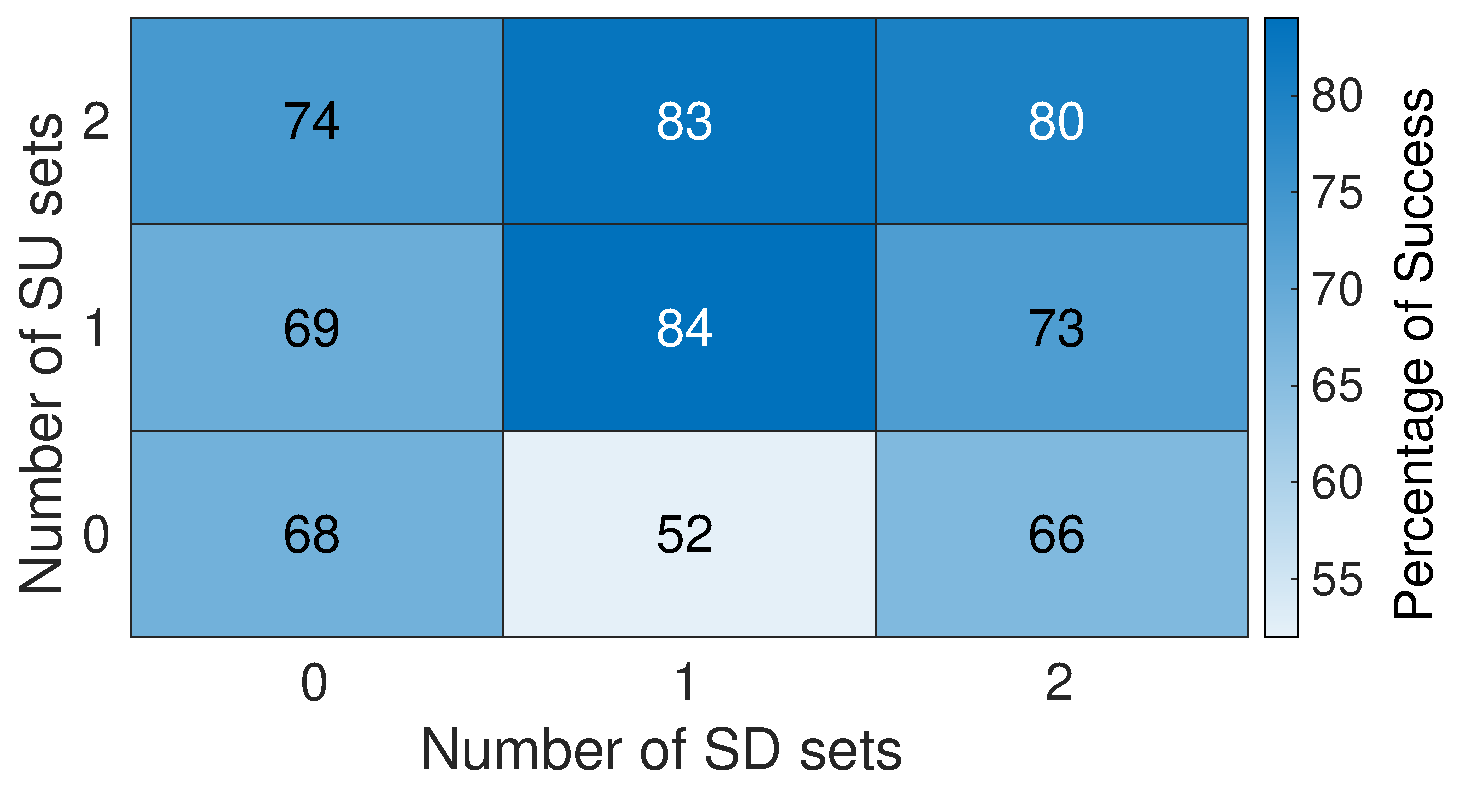
\includegraphics[width=0.65\linewidth]{NAB2_heatmap}
	\caption{Estimator performance for a user with SCI for chosen novel data.}\label{fig:heatmap}
\end{figure}

Steady-state walking in trials of subjects with iSCIs had a standard deviation of up to 0.18 m/s for their walking speed compared to 0.1 m/s seen in healthy users walking without robot assistance \cite{socie2013gait}. In addition to the severity of the iSCI, variability can be affected by user fatigue, discomfort, or misfit orthoses. As a result, some walking trials better represent the exoskeleton user's gait patterns than other trials performed on the same day. Therefore, choosing the appropriate training datasets from injured users is important to reduce noise in the data and accurately capture their gait patterns. Figure~\ref{fig:heatmap} shows the differences in accuracy of different estimator configurations in predicting gait speed changes. Each of these configurations used the same base data but different novel training data from a combination of a number SU/SD trials as listed on the axes. Estimator accuracy differs based on the novel data used for customization, so these data must be chosen carefully. This choice may be increasingly difficult to make as the number of trials to consider increases. 

One way to make this choice is to consider the Mutual Information (MI) between the measured variables (gait features) and those to be inferred (desired speed). MI is a measure of the information obtained about one random variable by observing another variable \cite{cover1999elements}. The MI between two variables may be computed using the Kullback-Leibler (KL) divergence, $ D_{KL} $, between their joint and marginal distributions. For example, consider two distributions $ A $ and $ B $ of an arbitrary variable $ x $. The KL divergence $ D_{KL}(A||B) $ is a measure of how different the two distributions are, as illustrated in Fig.~\ref{fig:divergence}. The mutual information between the two variables $ A $ and $ B $ is $ I(A;B) = D_{KL}(p_{(A,B)}||p_A p_B) $ where $ p_{(A,B)} $ is their joint probability and $ p_A $ and $ p_B $ are their marginal probabilities. Roughly, the MI provides a scalar measure of the correlation between the two variables.
%
\begin{figure}
	\centering
	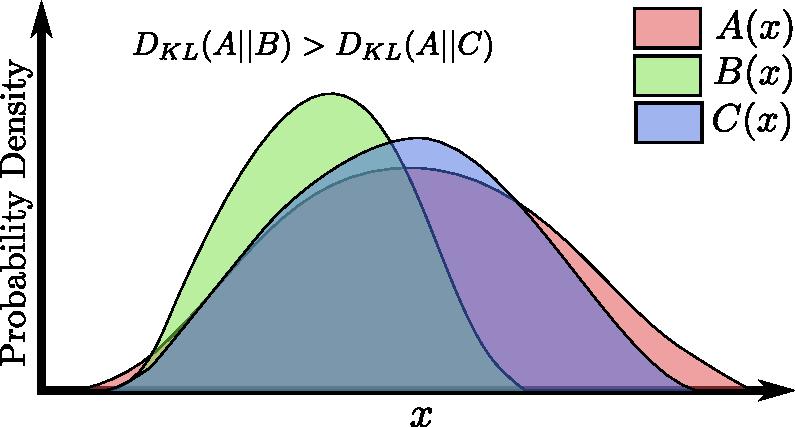
\includegraphics[width=0.6\linewidth]{divergence.pdf}
	\caption{The difference between two distributions may be quantified using KL divergence.}\label{fig:divergence}
\end{figure}

The computation of KL divergence is simplified with the assumption that both distributions are Gaussian. The KL divergence between distributions $ A \sim \mathcal{N}\left(\mmu_a, \Ssigma_a\right) $ and $ B \sim \mathcal{N}\left(\mmu_b, \Ssigma_b\right) $ is given by

\begin{equation}
	D_{KL} (A||B) = \int_{x} P_A(x) \log \frac{P_A(x)}{P_B(x)}dx \label{eq:kl_def}
\end{equation}
%
with the probability density function of a generic multivariate Gaussian random variable $ \x \in \mathbb{R}^k$ with mean $ \mmu \in \mathbb{R}^k $ and covariance $ \Ssigma \in \mathbb{R}^{k \times k}$ given by
%
\[
	p(\x) = \frac{1}{(2\pi)^{k/2} |\Ssigma|^{1/2}} \exp\left(-\frac{1}{2} (\x-\mmu)^T \Ssigma^{-1} (\x-\mmu)\right)
\]
%
%The expected value of a random variable $ X $ is defined as \[\mathbb{E}[X] = \int_{-\infty}^{\infty} x f(x) dx\] therefore, using \eqref{eq:kl_def}, KL divergence may be defined as
%\begin{eqnarray}
%	D_{KL}(A||B) &=&  \mathbb{E}_A \left[\log \frac{A}{B}\right] \nonumber \\
%	{} &=& \mathbb{E}_A \left[\log(A) - \log(B)\right] \label{eq:dkl_exp}
%\end{eqnarray}
%%
Substituting the probability density functions of $ A $ and $ B $ into \eqref{eq:kl_def}, the computation of $ D_{KL}(A||B) $ is simplified \cite{duchi2007derivations} to
%
\begin{equation}
	D_{KL}(A||B) = \frac{1}{2} \left[\log \frac{|\Ssigma_b|}{|\Ssigma_a|} - k + (\mmu_a - \mmu_b)^T \Ssigma_b^{-1} (\mmu_a - \mmu_b) + tr\{\Ssigma_b^{-1} \Ssigma_a\} \right] \label{eq:dkl}
\end{equation}
%
where $ tr\{\Ssigma_b^{-1} \Ssigma_a\} $ is the trace of $\Ssigma_b^{-1} \Ssigma_a $. As $ p_{(A,B)} $ and $ p_A p_B $ have the same dimension, mean, and diagonal of the covariance matrix when computing the MI, the computation of $ I(A;B) $ using \eqref{eq:dkl} further simplifies down to
\begin{equation}
	I(A;B) =\frac{1}{2} \left[\log \frac{|\Ssigma_{ab}^{'}|}{|\Ssigma_{ab}|} \right] \label{eq:MI}
\end{equation}
where $ \Ssigma_{ab} = E[(A - \greekvec{\mu}_a)(B - \greekvec{\mu}_b)^T] $ and $ \Ssigma_{ab}^{'} $ is a block diagonal matrix with the cross-covariance between $ A $ and $ B $ in $ \Ssigma_{ab} $ set to zero. Roughly, the MI provides a scalar measure of the correlation between the two variables.	

MI was used to measure the utility of the measured gait features for estimating the desired gait speed. Since the true desired gait speed is difficult to determine, the speed at the next step, denoted $ v' $, was assumed as its proxy, similar to Chapter~\ref{chapter:BKF}. The distributions of gait speed and features were approximated as Gaussian and the MI $ I(V ; Q) $ was computed, where $ V $ is the distribution of the step-to-step changes in desired speed estimated via $ \Delta v' $, and $ Q $ is the distribution of the corresponding changes in gait feature measurements from step-to-step, estimated from $ \Delta \Q $. The intuition behind using distributions of the changes in gait speed and features is to incorporate the knowledge of their evolution through intent changes into the selection process. 

To avoid training the estimator on all available speed change data and leave some data for testing, the novel training dataset was limited to at most three out of all available trials for each injured user. Combinations of available novel trial data were generated by choosing two or three out of the available number of trials and collected in a set $ W $. The MI was computed for the novel/base data pairing for each combination in the set, stored in a vector $ \greekvec{\iota} \in \mathcal{R}^{{\rm len}(W)}$. The pairing with the highest MI was chosen. Algorithm \ref{algo:selection} details this overall process to select the appropriate novel trial data for augmenting the base data.

\begin{algorithm}
	\caption{Training set selection}\label{algo:selection}
	\begin{algorithmic}[1]
		\Require $ \v'_n$, $\v'_b $, $ \Q_n $, $\Q_b$
		\State {\em Note:} $ W $ denotes a set where each element is a combinations of novel trials to be considered
		\For{$ m = 1 $ to $ {\rm len}(W) $}
		\State $ \v'_{n/b} = (\v'_b - \bar{v}'_b)\sigma_{v'_n} \sigma_{v'_b}^{-1} + \bar{v}'_n $ 
		\State $ \v' \leftarrow [\v_{n/b}^{'T}\ \v_{n}^{'T}]^T $
		\For{$ s = 1 $ to $ S $}
		\State $ \q_{n/b} = (\q_b - \bar{q}_b)\sigma_n \sigma_b^{-1} + \bar{q}_n $ 
		\State $ \q \leftarrow [\q_{n/b}^T\ \q_{n}^T]^T $
		\EndFor
		\State $ \Q = [\q_1 \ \q_2 \dots \q_S] $
		\State $ \v' \leftarrow \Delta \v' $
		\State $ \Q \leftarrow \Delta \Q $
		\vskip 5pt
		\State $ \begin{bmatrix}
			Q \\
			V
		\end{bmatrix} \sim \mathcal{N} \left( \begin{bmatrix}
			\bar{\q} \\
			\bar{v}'
		\end{bmatrix},\begin{bmatrix}
			\Ssigma_{\q \q} & \Ssigma_{\q v'} \\
			\Ssigma_{v' \q} & \Sigma_{v'v'}
		\end{bmatrix}\right) $
		\vskip 2pt
		\State $ \iota_m = I(V;Q) $
		\EndFor
		\State \Return $m$ such that $\iota_m$ = $ \max(\greekvec{\iota}) $ 
	\end{algorithmic}
\end{algorithm}%

\subsection{Estimating the Desired Gait Velocity}\label{sec:models}

Gait features and desired speed were assumed to follow Gaussian distributions during estimation as well. In contrast to Chapter~\ref{chapter:BKF}, let the desired gait speed $ v^d $ be rewritten as $ z $ to simplify notation:
\begin{align}
	\begin{bmatrix}
		\q \\
		z
	\end{bmatrix} &\sim \mathcal{N}\left(\begin{bmatrix}
		\bar{\q} \\
		\bar{z}
	\end{bmatrix},
	\begin{bmatrix}
		\Ssigma_{\q \q} & \Ssigma_{\q z} \\
		\Ssigma_{z \q} & \Sigma_{z z}
	\end{bmatrix}\right) \label{eq:full_dist}
\end{align}
where the means and covariances were computed using the training data that includes both base and novel data. Given measurements $\tilde{\q}$ of the gait features at TD, the estimated mean and variance of the desired gait speed, for the first stage of the BKF, were determined using standard conditional probability equations
\begin{align}
	\hat{z} &= \bar{z} + \Ssigma_{z \q} \Ssigma_{\q \q}^{-1} \left(\tilde{\q} - \bar{\q}\right) \label{eq:v_up} \\	
	\hat{\Sigma}_{z z} &= \Sigma_{z z} - \Ssigma_{z \q} \Ssigma_{\q \q}^{-1} \Ssigma_{\q z} \label{eq:c_up}
\end{align}

The estimate $\hat{z}$ is driven by the error between the training mean $ \bar{\q} $ and gait feature measurements $ \tilde{\q} $. Along with $\hat{z}$, the resulting estimator outputs an SU/SD signal at TD as the difference between $ \hat{z} $ at the current and previous TD. A speed change threshold for a SU/SD was determined by recording the standard deviation in step-to-step speed changes observed from three steady-state walking steps from each trial in the training data. This threshold is important due to the minimal detectable change (MDC) or the minimal change in the measured gait speed required to distinguish between a true change and noise. The MDC for people with iSCIs was shown to be around 0.17~m/s \cite{mohandas2012minimal}.

\section{Results \& Discussion} \label{sec:results}

The performance of data pooling for crutch and walker-assisted walking was evaluated on experimental data (Section~\ref{sec:exoData}) and the efficacy of the algorithm was explored as described in Section~\ref{sec:efficacy}. Initial testing involved using base and novel data from trials using the same ambulatory device, i.e., walker or crutches as presented in Sections~\ref{sec:ww}~and~\ref{sec:cc}. Additional testing was then performed to explore the interchangeability of base data to explore the effects of these ambulatory devices on gait patterns and estimator performance and is described in Section~\ref{sec:interchangeability}.

\subsection{Testing on walking trial data}
One step before and three steps after the speed change command, for a total of four steps, were chosen as training data from all base and novel trials. For each ambulatory device, i.e., crutches or walker, the base data consisted of 6 trials from each uninjured user in each mode, adaptive and free, for a total of 72 trials. While similar user responses to desired speed change exist for free and adaptive mode, they are evident in different sensor measurements, as described in the previous chapter. Despite these differences, more base data was found to result in improved accuracy, even when that data resulted in a mode mismatch between base and novel data. For example, for IU-1, excluding base data from trials in free mode resulted in an estimator accuracy of 69\% compared to 80\% when both free and adaptive mode data were included in the base set. Up to three trials (i.e., 12 steps' worth of data) were selected as novel data for each injured user via Algo.~\ref{algo:selection} and used to transform the base data. The estimator was then run on all available trial data for each subject (38-85 steps) out of which at most 12 steps were seen in training. The estimated change in desired speed was compared to the measured change, and if the speed change sign was correctly anticipated, it was considered a successful estimate.

Figure~\ref{fig:single_trial} visualizes the output of the estimator for an SD trial with IU-1 where the dashed black lines illustrate the speed change threshold used to determine true changes. While the intent signal is represented similarly as in the previous chapter, the accuracy of $ \hat{z} $ was found to be comparatively better due to the revisions to estimator described in this Chapter. Therefore, similarly to Section~\ref{sec:add_analysis}, the RMS error between the predicted gait speed change at TD and the value measured at the subsequent MS was considered while evaluating estimator performance. 

\begin{figure}
	\centering
	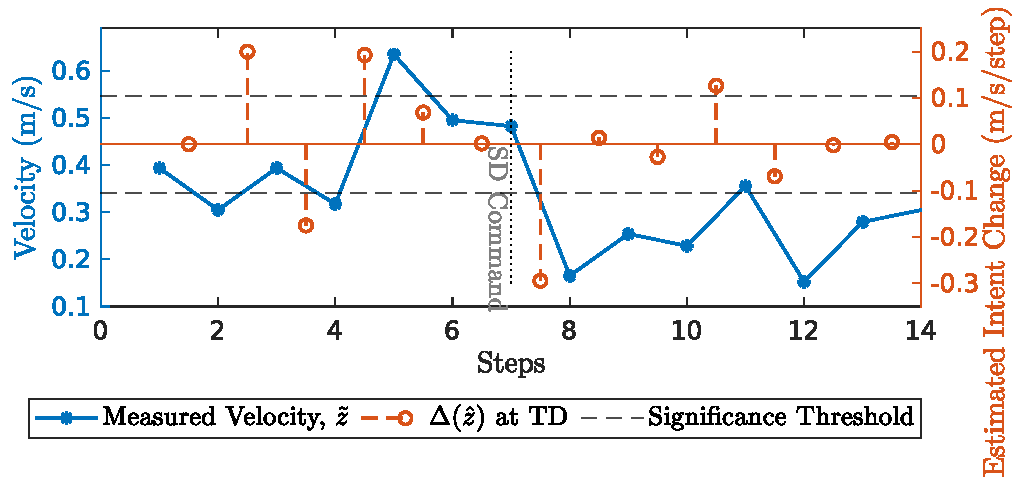
\includegraphics[width=0.9\linewidth]{single_trial.pdf}
	\caption{Output of a single estimator trial for IU-1.}\label{fig:single_trial}
\end{figure}

The  estimator was run in three configurations for both subjects to highlight the benefits of using both novel and base data, as illustrated in Fig.~\ref{fig:novel_comp}. The confusion matrix for the trials of IU-2 is listed in Table~\ref{table:comp_table}. The color of each cell ranges from green to red as the accuracy ranges from 100\% to 0\% therefore, the higher the accuracy, the greener the cell. The base data was from walker trials and the novel data was from walker and crutch trials for IU-1 and IU-2, respectively. The first configuration used untransformed base data (Base\textsubscript{b}), the second used only the transformed base data (Base\textsubscript{n/b}), and the third used both novel and transformed base data (Novel+Base\textsubscript{n/b}). Minor increases in SU/SD identification accuracy were observed (Fig.~\ref{fig:novel_comp}) when using only the transformed base data, as the accuracy depends on identifying only the speed changes, and not their magnitude. Despite increases in accuracy, the RMS errors deteriorated and were unacceptable at 12.8 m/s and 3.6 m/s for IU-1 and IU-2 respectively. Adding novel data to the transformed base data increased the speed change estimation accuracy and decreased the RMS errors. 

\begin{figure}
	\centering
	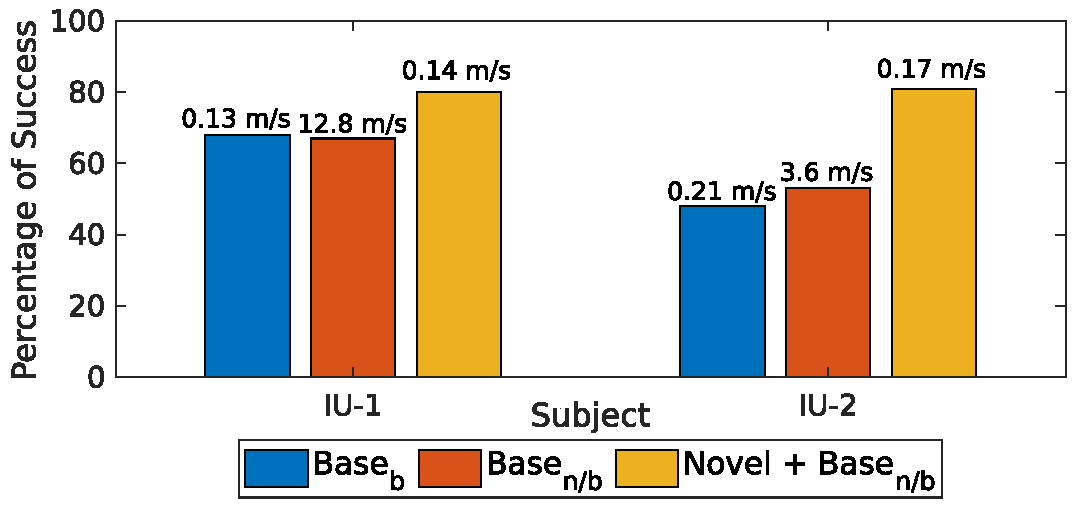
\includegraphics[width=0.8\linewidth]{novel_comp.pdf}
	\caption{Percentage of success with and without novel data for both subjects, labeled with RMS error between predicted and measured gait speed changes.}\label{fig:novel_comp}
\end{figure}

\begin{table}
	\centering
	\caption{Confusion matrix for IU-2 \\ For estimation with and without novel data }\label{table:comp_table}
	\begin{tabular}{|c|c|c|c|c|c|c|}
	\hhline{-------}
	& \multicolumn{3}{c|}{Predicted SD} & \multicolumn{3}{c|}{Predicted SU} \\ 
	\hhline{~------}
	& Base \textsubscript{b} & Base \textsubscript{n/b} & Novel & Base \textsubscript{b} & Base \textsubscript{n/b} & Novel \\
	\hhline{-------}
	Actual SD	& \prescolor{50} & \prescolor{51} & \prescolor{78} & \frescolor{53} & \frescolor{45} & \frescolor{17} \\ %\hhline{---} %6/ & 8/3
	\hline
	Actual SU	&  \frescolor{50} & \frescolor{49} & \frescolor{22} & \prescolor{47}& \prescolor{55} & \prescolor{83} \\ \hhline{-------}%6/ & 7/9
	%			\hline 
\end{tabular}
\end{table}

The trials of IU-1 using only base data had an overall success rate of 68\%. Upon using novel data, the success rate increased to 80\% with a p-value $ p = 0.049$ where the null hypothesis was that the success rate would stay the same. Similarly, the success rate for IU-2 increased from 48\% to 80\% with a p-value $ p = 7\times10^{-5} $. Therefore, using novel data resulted in statistically significant increases in accuracy.

\subsection{Efficacy of the Novel Data Selection Algorithm}\label{sec:efficacy}

The number of possible combinations of novel data in Algo. \ref{algo:selection} for training was 35 for walker trials and 12 for trials with crutches for IU-1. There were fewer trials with walking using crutches, as there was data loss from sensors that hindered the identification of gait events. All combinations of these trials were used as novel data with base data from uninjured subjects using a walker to train conditional models that were used in the estimator. The percentages of success of those estimator trials are shown in Fig.~\ref{fig:rand_box}. The whiskers denote the most extreme points, and the central line denotes the median. The green markers illustrate the success rates observed when the novel data chosen using Algo.~\ref{algo:selection} was used. If novel data is chosen at random, accuracy may be as low as 59\%, however, using the novel data selection algorithm outlined previously ensures a high likelihood of increased success despite not guaranteeing it. The difference between the results shown in green and the maximum success rate shown by the top whisker would be of at most four misclassified steps for both, crutch and walker trials. The increase in accuracy seen in Figure~\ref{fig:novel_comp} after pooling novel and base data further highlights the importance of including user-specific data.

Overall, our analysis showed different outcomes based on the assistive device used in the novel data. This observation motivates the remainder of the analysis herein, which considers the effects of the assistive device on the efficacy of our methods. 

\begin{figure}
	\centering
	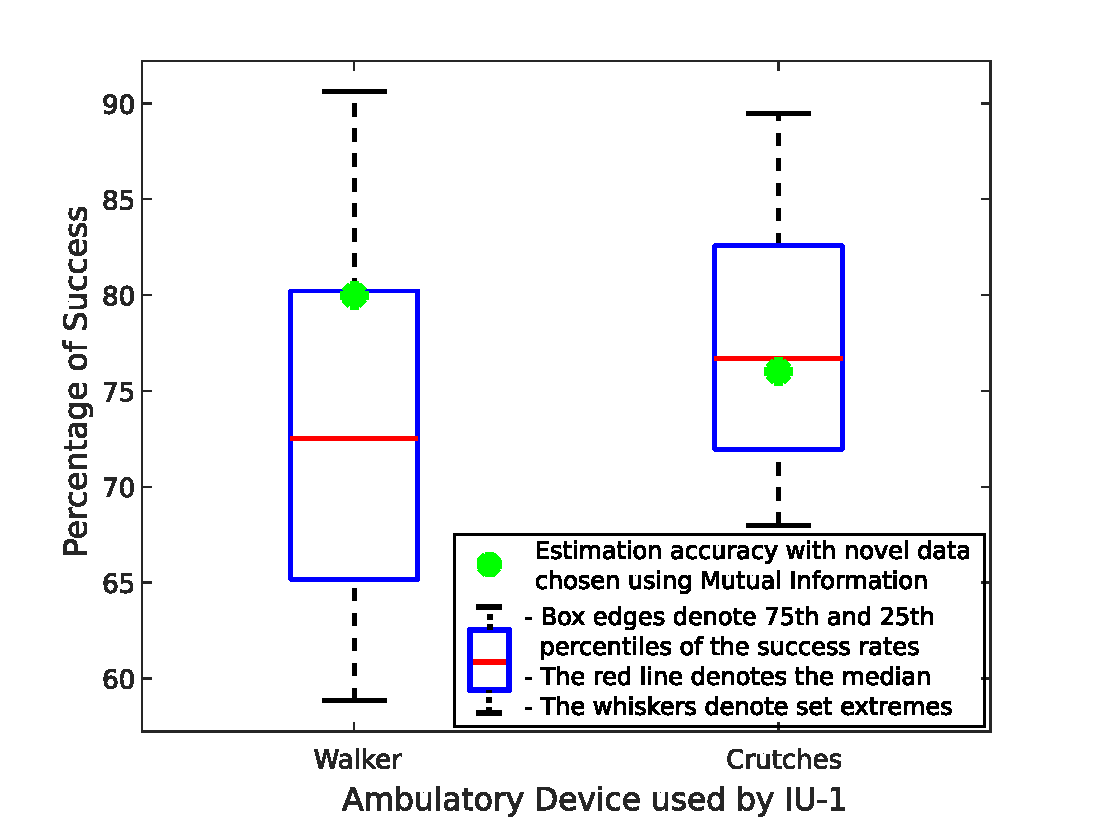
\includegraphics[width=0.86\linewidth]{rand_box_new.pdf}
	\caption{Percentage of success for IU-1 with the base data from walker trials and the novel dataset chosen randomly vs. using Algo. \ref{algo:selection}.}\label{fig:rand_box}
\end{figure}

\subsection{Walking Trials Using Walker}\label{sec:ww}
Estimation for both IU-1 and IU-2 was first performed using base data exclusively from walking trials of uninjured users using walkers. The performance for these users is summarized by the confusion matrix in Table~\ref{table:confmat_w_w}. The estimator for IU-1 was personalized using one SD and two SU trials. The speed change threshold for this estimator configuration was 0.072 m/s, i.e., if the change in predicted speed at TD compared to the measured speed at the previous MS was smaller than this threshold, the SU/SD prediction was ignored. Walking trials for IU-1 had 90 steps, 46 having significant speed changes. 80\% of SU and 81\% of SD changes were accurately detected at TD, for an overall accuracy of 80\% with an RMS speed error of 0.14 m/s.

\begin{table}
	\centering
	\caption{Confusion matrix for \\Novel Data - Walker/Base Data - Walker}\label{table:confmat_w_w}
	\begin{tabular}{|c|c|c|c|c|}
		\hhline{-----}
		& \multicolumn{2}{c|}{Predicted SD} & \multicolumn{2}{c|}{Predicted SU} \\ 
		\hhline{~----}
		& IU-1 & IU-2 & IU-1 & IU-2 \\
		\hhline{-----}
		Actual SD	& \prescolor{80} & \prescolor{58} & \frescolor{19} & \frescolor{78} \\ %\hhline{---} %6/ & 8/3
		\hline
		Actual SU	&  \frescolor{20} & \frescolor{42} & \prescolor{81}& \prescolor{22} \\ \hhline{-----}%6/ & 7/9
		%			\hline 
	\end{tabular}
\end{table}

Similarly for IU-2, the change threshold was 0.13 m/s. Out of the 73 total steps, 21 had significant speed changes, and 58\% SD and 22\% SU changes were accurately detected at TD for an overall accuracy of 43\%. The confusion matrix is given in Table~\ref{table:confmat_w_w}. These trials had higher gait variability as seen from the standard deviation of the steady-state velocity of 0.13 m/s compared to 0.072 m/s for IU-1, which may explain the difficulty in estimation and drop in success rate. Preliminary work suggests other methods to address this low success rate, which are discussed at the end of this section.

\subsection{Walking Trials Using Crutches}\label{sec:cc}

The choice of the assistive device affects gait patterns, so estimation was performed for both injured users for walking trials using crutches with the performance summarized in Table~\ref{table:confmat_c_c}. The base data contained walking trials of uninjured users exclusively using crutches. The speed change threshold was 0.11 m/s. There were 4 significant speed changes in the trials for IU-1, out of which 3 were detected successfully for an overall success rate of 75\% with an RMS error of 1.52 m/s. The success rates of SU and SD are shown in Table~\ref{table:confmat_c_c}.

\begin{table}
	\centering
	\caption{Confusion matrix for \\Novel Data - Crutches/Base Data - Crutches}\label{table:confmat_c_c}
	\begin{tabular}{|c|c|c|c|c|}
		\hhline{-----}
		& \multicolumn{2}{c|}{Predicted SD} & \multicolumn{2}{c|}{Predicted SU} \\ 
		\hhline{~----}
		& IU-1 & IU-2 & IU-1 & IU-2 \\
		\hhline{-----}
		Actual SD	& \prescolor{100} & \prescolor{85} & \frescolor{33} & \frescolor{22} \\ 
		\hline
		Actual SU	&  \frescolor{0} & \frescolor{15} & \prescolor{67}& \prescolor{78} \\ \hhline{-----}
		%			\hline 
	\end{tabular}
\end{table}

The trials for IU-2 had 75 steps, out of which 36 had significant speed changes with a threshold speed of 0.1~m/s. The percentage of success was 81\% with 29 speed changes correctly identified and the rates for SU and SD changes are shown in Table~\ref{table:confmat_c_c}. The RMS error of the speed estimates was 0.2 m/s. A possible explanation for the lower estimator performance for IU-1 is that there may not be enough information about the desired gait speed in the user's gait patterns as evidenced by the amount of MI in the data. The values of MI for the selected novel data for IU-1 and IU-2 were 0.3 and 0.39 respectively. The difference in the $ \iota $ of the two pairings indicates that the gait feature measurements for IU-2 carried roughly 30\% more information about the intended speed than those for IU-1 in this case.

\subsection{Exploring the Interchangeability of Base Data}\label{sec:interchangeability}

Interchangeability of base data was studied to explore the effect of ambulatory devices on estimator accuracy by using different devices for the novel and base data. The first pairing was for IU-1 where the novel data was from trials using crutches and base data was from trials using a walker. The overall success rate for this trial, with 17 significant speed changes, was 76\% and the RMS error was 0.09 m/s. The confusion matrix for this trial is listed in Table~\ref{table:confmat_c_w}. Estimation performed on trial data of IU-2 walking using crutches with base data from trials using a walker yielded a percentage of success of 80\% and an RMS error of 0.17 m/s with the confusion matrix also given in Table~\ref{table:confmat_c_w}. 

\begin{table}
	\centering
	\caption{Confusion matrix for \\Novel Data - Crutches/Base Data - Walker}\label{table:confmat_c_w}
	\begin{tabular}{|c|c|c|c|c|}
		\hhline{-----}
		& \multicolumn{2}{c|}{Predicted SD} & \multicolumn{2}{c|}{Predicted SU} \\ 
		\hhline{~----}
		& IU-1 & IU-2 & IU-1 & IU-2 \\
		\hhline{-----}
		Actual SD	& \prescolor{78} & \prescolor{78} & \frescolor{25} & \frescolor{17} \\ 
		\hline
		Actual SU	&  \frescolor{22} & \frescolor{22} & \prescolor{75}& \prescolor{83} \\ \hhline{-----}
		%			\hline 
	\end{tabular}
\end{table}

These results were compared to estimator trials with IU-1 in which the base data and novel data were both from walking trials with crutches. In this case, the success rate and RMS error were 75\% and 1.52 m/s respectively. Surprisingly, this overall success rate was similar and the RMS error was higher than when the base data was from trials with a walker as in the previous paragraph. Further analysis revealed that the task of gait speed estimation was particularly difficult for IU-1 with crutches since  32 of the 38 steps were below the MDC threshold of 0.17 m/s found in literature. In both of the previous cases, the novel data was the same, only the base data was changed. However, pairing the novel data with walker and crutch base data results in MI values of 0.4048 and 0.3007 respectively, so gait features are more informative of gait speed when uninjured users use a walker. As a result, the model generated using base data from walker trials was able to handle the increased estimation difficulty and increase the estimator accuracy and lower RMS error. This result highlights the flexibility of the estimator to incorporate the most informative base data, even under potentially mismatched conditions.

However, this interchangeability did not hold for every pairing. Estimation was performed for IU-1 with novel data from walking trials with a walker and base data from trials with crutches. Compared to estimation using base data from trials with a walker, the percentage of success dropped to 63\% with an RMS error of 0.12 m/s, and the confusion matrix for this trial is given in Table~\ref{table:confmat_w_c}. There was a less severe deterioration in performance for IU-2. The success rate and RMS error were 38\% and 0.26 m/s, respectively; a difference of 5\% and 0.046 m/s  when  compared to the performance of the same novel data paired with data of trials with a walker (see Section \ref{sec:ww}). 

\begin{table}
	\centering
	\caption{Confusion matrix for \\Novel Data - Walker/Base Data - Crutches}\label{table:confmat_w_c}
	\begin{tabular}{|c|c|c|c|c|}
		\hhline{-----}
		& \multicolumn{2}{c|}{Predicted SD} & \multicolumn{2}{c|}{Predicted SU} \\ 
		\hhline{~----}
		& IU-1 & IU-2 & IU-1 & IU-2 \\
		\hhline{-----}
		Actual SD	& \prescolor{67} & \prescolor{50} & \frescolor{45} & \frescolor{75} \\ 
		\hline
		Actual SU	&  \frescolor{33} & \frescolor{50} & \prescolor{55}& \prescolor{25} \\ \hhline{-----}
		%			\hline 
	\end{tabular}
\end{table}

In general, estimators had higher percentages of success across all tests when using base data of walker trials. This may be as the crutches offer more freedom to move during use than a walker, resulting in more individualized effects on gait patterns across trials. Again, the lower correlation between gait speed and features is evidenced by the MI in the untransformed walker base data (0.3675) being higher than the  crutch base data (0.2813), so gait features are more informative of gait speed when uninjured users use a walker. These inconsistencies could possibly be overcome by adding instrumentation such as IMUs \cite{brescianini2011ins} to crutches to capture their role in gait dynamics. Additionally, upon expanding the base dataset to include both crutch and walker trials, estimator performance either stayed the same or deteriorated. This deterioration is seen when comparing the estimator performance in Tables~\ref{table:confmat_w_w}~and~\ref{table:confmat_w_wc} where the overall accuracy dropped from 80\% to 61\% and the RMS error increased from 0.14 m/s to 0.19 m/s. In the case of IU-2, comparing Tables~\ref{table:confmat_c_c}~and~\ref{table:confmat_c_wc}, the estimator performance is similar with accuracies of 81\% each and RMS errors of 0.17 m/s and 0.16 m/s respectively. These results suggest that choosing subsets of the base data along with novel data (e.g., using extensions of Algo.~\ref{algo:selection}) may allow further improvement in estimator performance.

\begin{table}
	\centering
	\caption{Confusion matrix for \\Novel Data - Walker/Base Data - Walker \& Crutches}\label{table:confmat_w_wc}
	\begin{tabular}{|c|c|c|c|c|}
		\hhline{-----}
		& \multicolumn{2}{c|}{Predicted SD} & \multicolumn{2}{c|}{Predicted SU} \\ 
		\hhline{~----}
		& IU-1 & IU-2 & IU-1 & IU-2 \\
		\hhline{-----}
		Actual SD	& \prescolor{60} & \prescolor{43} & \frescolor{33} & \frescolor{67} \\ 
		\hline
		Actual SU	&  \frescolor{40} & \frescolor{57} & \prescolor{67}& \prescolor{33} \\ \hhline{-----}
		%			\hline 
	\end{tabular}
\end{table}

\begin{table}
	\centering
	\caption{Confusion matrix for \\Novel Data - Crutches/Base Data - Walker \& Crutches}\label{table:confmat_c_wc}
	\begin{tabular}{|c|c|c|c|c|}
		\hhline{-----}
		& \multicolumn{2}{c|}{Predicted SD} & \multicolumn{2}{c|}{Predicted SU} \\ 
		\hhline{~----}
		& IU-1 & IU-2 & IU-1 & IU-2 \\
		\hhline{-----}
		Actual SD	& \prescolor{100} & \prescolor{91} & \frescolor{50} & \frescolor{24} \\ 
		\hline
		Actual SU	&  \frescolor{0} & \frescolor{9} & \prescolor{50}& \prescolor{76} \\ \hhline{-----}
		%			\hline 
	\end{tabular}
\end{table}

Overall, pooling base and novel data improved estimator accuracy in every case except for trials of IU-2 using a walker. This loss of accuracy was due to noisy measurements during those particular trials. The traces of the model covariance matrices when using novel walker and crutch data were 3.425 and 2.015 respectively (for the same base data). Preliminary work shows that this noise in the IU-2 walker data can be attributed to certain noisy features for this user. Multiple gait features often provide the same information about gait speed while introducing unique noise. In such cases, using a reduced, minimally-redundant set of gait features \cite{peng2005feature} offers the potential to further improve accuracy. Preliminary results addressing this aspect show increases of over 20\% in overall estimation accuracy of the IU-2 trials shown in Tables~\ref{table:confmat_w_w}~and~\ref{table:confmat_w_c}. 

For IU-2, estimation was first performed using novel and base data from walker trials. Four minimally redundant features were selected, namely, the step length, the angle and angular velocity of the swing leg, and the angular velocity of the knee of the stance leg. The overall percentage of success increased from 43\%, as seen in Section~\ref{sec:ww}, to 79\% and the RMS error decreased from 0.21 m/s to 0.13 m/s. The confusion matrix for these trials is listed in Table~\ref{table:confmat_wc_red} where the columns show results with different base data pairings. Similarly, when using walker novel data and crutch base data, the only one feature, the time-to-touchdown (tTD), was selected. The overall percentage of success increased from 38\%, as seen in Section~\ref{sec:interchangeability}, to 67\% and the RMS error decreased from 0.26 m/s to 0.19 m/s. 

\begin{table}
	\centering
	\caption{Confusion matrix for IU-2 Walker Trials\\ Using a Reduced Feature Set and Varying Base Data}\label{table:confmat_wc_red}
	\begin{tabular}{|c|c|c|c|c|}
		\hhline{-----}
		& \multicolumn{2}{c|}{Predicted SD} & \multicolumn{2}{c|}{Predicted SU} \\ 
		\hhline{~----}
		& Walker & Crutches & Walker & Crutches \\
		\hhline{-----}
		Actual SD	& \prescolor{80} & \prescolor{83} & \frescolor{25} & \frescolor{50} \\ 
		\hline
		Actual SU	&  \frescolor{20} & \frescolor{17} & \prescolor{75}& \prescolor{50} \\ \hhline{-----}
		%			\hline 
	\end{tabular}
\end{table}

\subsection{Limitations}

The training process assumed that the velocity at the next step was a reliable proxy for the user's desired speed at the current step.  This approach is likely a worse approximation in adaptive mode than in free mode due to the effects of human-robot coupling. However, it may still accurately capture the direction (SU/SD) of the desired speed change, which is the goal of this work.

The number of possible novel/base data pairings makes it difficult to manually choose a pairing to customize the estimator. The presented method automates that choice but it does not provide any guarantee that the selected pairing is the best possible option. This observation is further supported by the study  by Moolchandani et al.,~\cite{moolchandani2021design} where estimation performed with an unoptimized feature set had marginally lower error than when an optimized set was used. 

Data from walking trials of only two subjects with iSCIs were used to evaluate this data selection method. These were experienced users and that experience affects the pHRI during exoskeleton use, as their familiarity with the device may allow them to better predict device behavior and convey their intent more reliably than a novice user. Therefore, it would be beneficial in the future to acquire data from additional trials of both injured and uninjured users with varying degrees of usage proficiency to expand both the novel and base datasets.

Finally, it is noted that the presented results were all obtained in offline evaluation. Assessing methods for integrating the estimated intent into control is an interesting next step, beyond the scope of this dissertation, the details of which will have coupling with the intent signals present for real-time estimation.

\section{Summary} \label{sec:conclusion}
%
This chapter presented a data-driven method for personalized estimation of the intended gait speed of a novel exoskeleton user while addressing the scarcity of training data. Data scarcity is addressed by using a small amount of user-specific data to transform an easily accessible base dataset with data from walking trials of uninjured users. This method relies on commonalities in gait patterns observed across subjects and considers 18 gait features to estimate the user's desire to change speeds. A pairing of novel and base data that well represents the novel user's gait patterns is achieved using the Mutual Information between gait features and gait speed. Conditional Gaussians were used to construct an estimate of the desired speed, which was then used to infer SU/SD changes. In the future, this method may be extended to use the estimated magnitude of the speed change, though additional work may be required to improve the metric quality of the speed estimates. Human limitations on speed change perceptions would set a lower bound of roughly 0.2~m/s for the  accuracy that would be practically noticeable \cite{zhang2015investigation}.